\section{Implementation of virtual reality application}
\lstset{%
    % Basic design
    backgroundcolor=\color{editorGray!50},
    basicstyle=\footnotesize\ttfamily\mdseries,   
    frame=l,
    % Line numbers
    xleftmargin={0.75cm},
    numbers=left,
    stepnumber=1,
    firstnumber=1,
    numberfirstline=true,
    % Code design   
    keywordstyle=\color{blue!100}\bfseries,
    commentstyle=\color{commentsGreen!100},
    ndkeywordstyle=\color{editorGreen!100},
    stringstyle=\color{myFuchsia!100},
    % Code
    language=HTML5,
    alsolanguage=JavaScript,
    alsodigit={.:;},
    tabsize=2,
    showtabs=false,
    showspaces=false,
    showstringspaces=false,
    extendedchars=true,
    breaklines=true,        
    % Support for German umlauts
    literate=%
    {Ö}{{\"O}}1
    {Ä}{{\"A}}1
    {Ü}{{\"U}}1
    {ß}{{\ss}}1
    {ü}{{\"u}}1
    {ä}{{\"a}}1
    {ö}{{\"o}}1
}

\subsection{Project initialization}
Before project can be initialized, Node.js has to be installed on PC used for development. To start a new JavaScript project, \texttt{npm init} command is used through command line, on Windows operating system it's usually PowerShell and on Unix systems, terminal. The multi-step wizard appears to guide developer through the project initialization process. It will generate the \texttt{package.json} file that includes these parts:

\begin{itemize}
\item{Name - title of the project}
\item{Version - project version, using semantic versioning}
\item{Description - short project description}
\item{Entry point - central file of our JavaScript code, usually index.js}
\item{Test command - NPM script for testing}
\item{Git repository - link to version control repository where application's code is hosted}
\item{Keywords - used to better allocate the project within NPM packages search}
\item{Author - project author}
\item{License - project license}
\end{itemize}

In the end, MathworldVR's \texttt{package.json} file looks like this:

\begin{lstlisting}
{
  "name": "mathworldvr",
  "version": "0.0.1",
  "description": "Math world in WebVR, powered by A-frame.",
  "main": "src/index.js",
  "scripts": {
    "test": "echo \"Error: no test specified\" && exit 1"
  },
  "repository": {
    "type": "git",
    "url": "git+https://github.com/michaltakac/mathworld.git"
  },
  "keywords": [
    "webvr",
    "math",
    "aframe",
    "mathworld",
    "vr",
    "room-scale"
  ],
  "author": "Michal Takáč",
  "license": "MIT",
  "bugs": {
    "url": "https://github.com/michaltakac/mathworld/issues"
  },
  "homepage": "https://github.com/michaltakac/mathworld#readme"
}
\end{lstlisting}

\subsection{Installing JavaScript packages}
In modern JavaScript development, applications are build by using many packages together. To install and use a package, developer first needs to search for one in NPM registry on \url{https://www.npmjs.com/}. Our application will need multiple packages. They are installed through command line with command \texttt{npm install <package-name>} found at the right side of every package detail web page:

\begin{figure}[ht!]
\centering
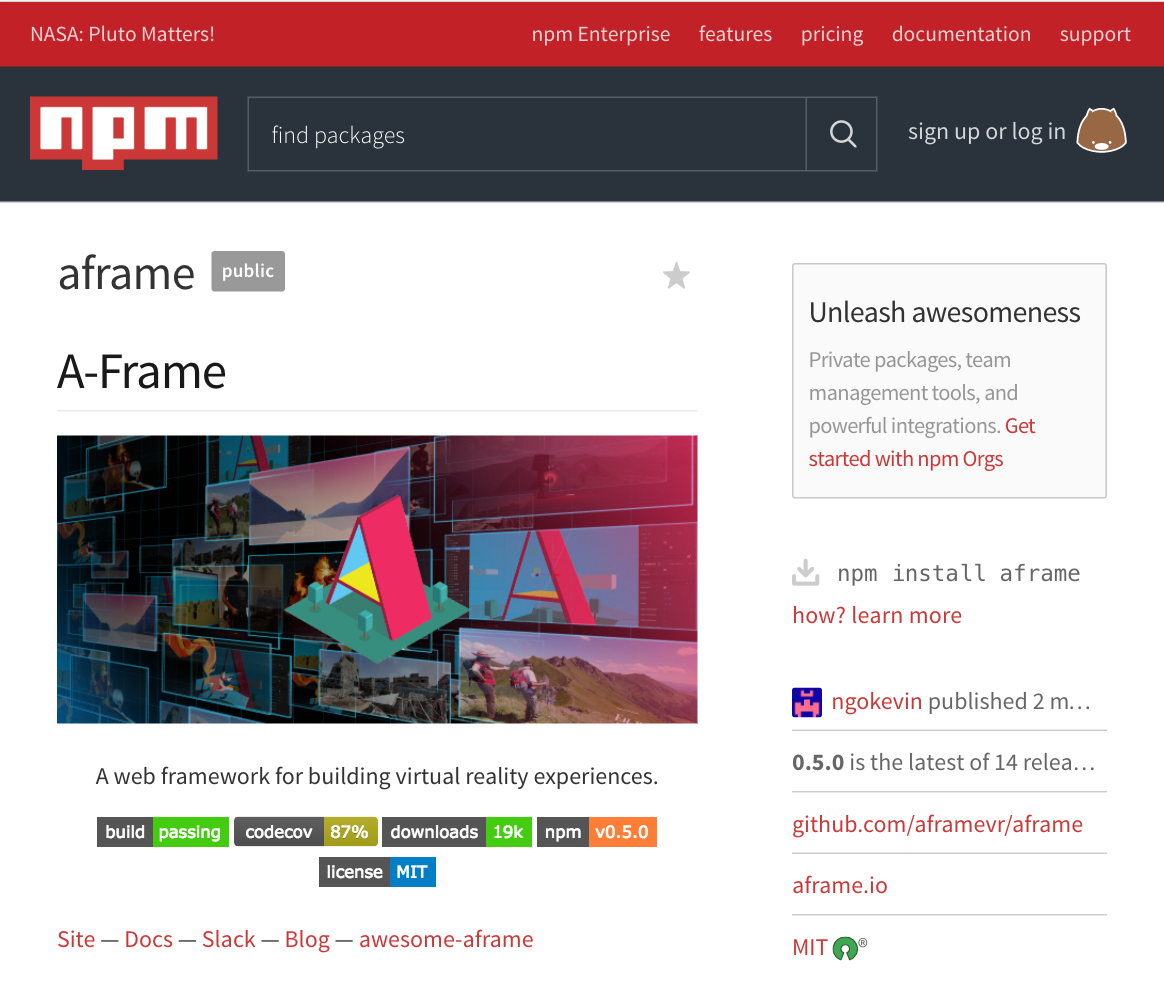
\includegraphics[width=0.9\textwidth]{npm-aframe}
\caption{Detail page of JavaScript package in NPM registry with the script to install highlighted.}
\label{r:61}
\end{figure}

To save a package into \texttt{package.json} file as a dependency, \texttt{--save} option has to be added to \texttt{npm install} command. To save it as a development dependency (only used for local development, doesn't get included in final build), we need to add \texttt{--save-dev} option instead. Packages with their respective version tag will be added to \texttt{package.json} file into specific location:

\begin{lstlisting}
"devDependencies": {
  "babel-cli": "^6.24.1",
  // ...
},
"dependencies": {
  "aframe": "^0.5.0",
  // ...
}
\end{lstlisting}

The list of used packages is included in System Manual.

\subsection{NPM scripts}
All of development, testing, bundling and deployment tasks are automated with \texttt{NPM scripts} defined in \texttt{package.json}.

\begin{lstlisting}
"scripts": {
  "start": "node server",
  "test": "jest",
  "test:watch": "npm test -- --watch",
  "coverage": "npm test -- --coverage && opn coverage/lcov-report/index.html",
  "lint": "eslint 'src/**/*.js' webpack.config.js server.js",
  "clean": "del 'build/!(.git*|Procfile)**'",
  "build:copy": "copyfiles -u 1 public/* public/**/* build",
  "build:clean": "rimraf \"build/!(.git*|Procfile)**\"",
  "prebuild": "npm run build:clean && npm run build:copy",
  "build": "cross-env NODE_ENV=production webpack"
},
\end{lstlisting}

\begin{itemize}
\item{"start" - Starts the development server.}
\item{"test" - Initialize Jest test runner that searches for all files that have \texttt{*.test.js} or \texttt{*.spec.js} in their file name and triggers all tests.}
\item{"test:watch" - Test runner will keep watching for file changes and will restart tests after every change.}
\item{"coverage" - Generates detailed test coverage report.}
\item{"lint" - Runs eslint for static code analysis testing according to preconfigured eslint rules in \texttt{.eslintrc}.}
\item{"clean" - Deletes the \texttt{/build} folder.}
\item{"build:copy" - Copies folders and files from \texttt{/public} into \texttt{/build}.}
\item{"build:clean" - Similar to "clean" command.}
\item{"prebuild" - Chain of NPM scripts that will be executed before actual "build" script.}
\item{"build" - Production-ready build that can be deployed to server.}
\end{itemize}

\subsection{Project structure}

\begin{figure}[ht!]
\centering
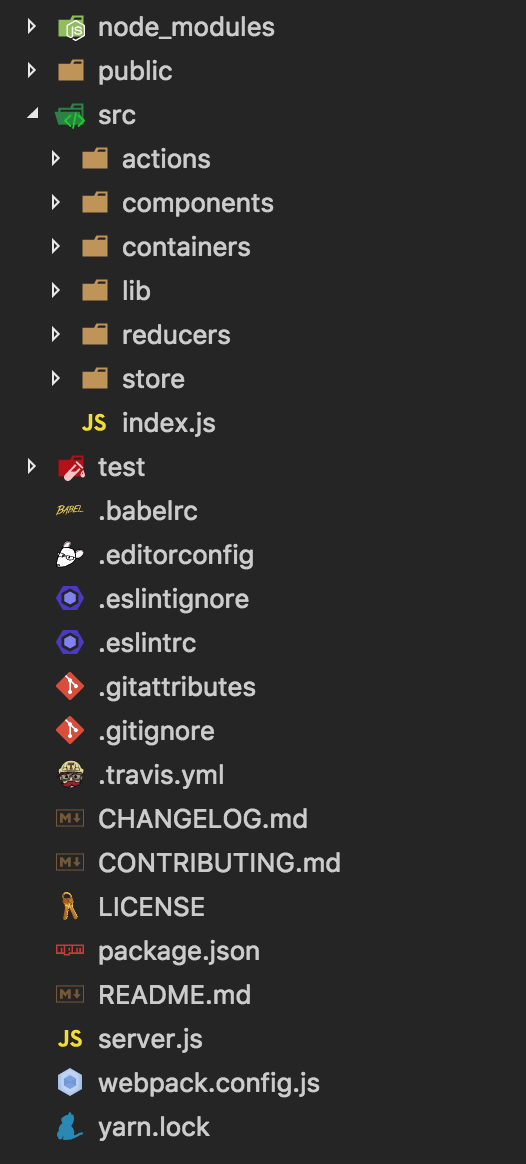
\includegraphics[width=0.3\textwidth]{folder-structure}
\caption{Project folder structure}
\label{r:62}
\end{figure}


\subsection{Webpack configuration}
Webpack is used as a tool to build JavaScript modules in MathworldVR application. It simplifies development workflow by quickly constructing a dependency graph of JavaScript application and bundling them in the right order. Our webpack configuration is defined in \texttt{webpack.config.js} and includes optimisations to the code like minification, obfuscation or splitting vendor/CSS/JavaScript code for production build. It also includes the configuration of Babel transpiler, which transpiles ES6/ES7 code to ES5, supported by all modern browsers.

\subsection{Webpack development server}
Development server configuration is defined in \texttt{server.js}. To start the server, \texttt{npm start} command is used from command line.

\begin{figure}[ht!]
\centering
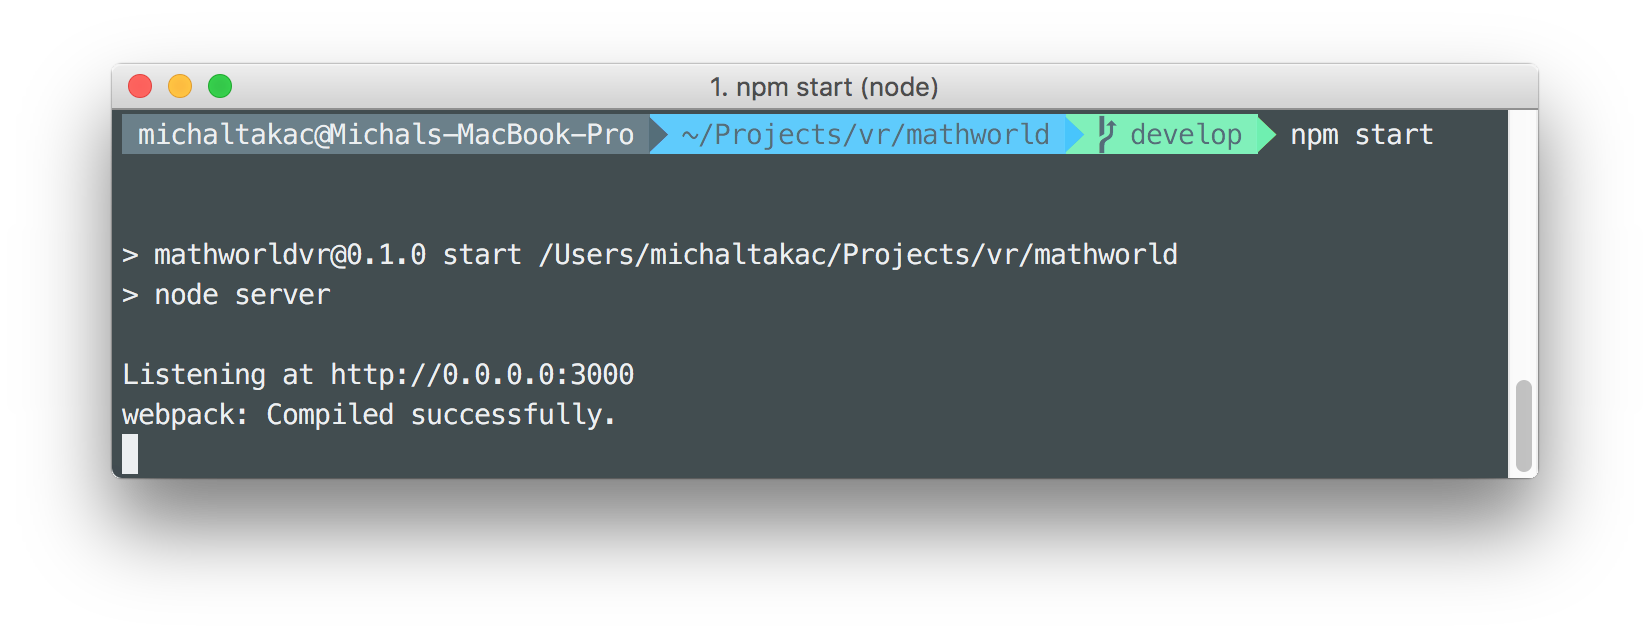
\includegraphics[width=0.9\textwidth]{npm-start}
\caption{Started development server.}
\label{r:63}
\end{figure}

\subsection{Setting up Redux for application state management}
In Redux, all the application state is stored as a single object. We need to think of its shape before writing any code. In MathworldVR, there are 5 main "features" -  \texttt{calculator}, interactable \texttt{function box} with grid, inside which resides the \texttt{parametric function} handling 3D visualization and \texttt{settings} for this visualization, represented by interactive settings panel. Each of those has it's own state. These are combined together into one, global state, including additional \texttt{user} state that represents user position and \texttt{ui} state that represents traditional 2D user interface behaviour, like the visibility of information panel displayed after MathworldVR page is rendered in browser. For each feature and additional state, one Reducer function exists and by using reducer composition, all reducers are combined together into one, root reducer. Code for reducer composition is defined in \path{src/reducers/index.js}.

\begin{lstlisting}[caption={Reducers composition code.},captionpos=b]
import { combineReducers } from 'redux'
import calculator from './calculator'
import functionBox from './functionBox'
import parametricFunction from './parametricFunction'
import settings from './settings'
import ui from './ui'

const rootReducer = combineReducers({
  calculator,
  functionBox,
  parametricFunction,
  settings,
  ui
})

export default rootReducer
\end{lstlisting}

\texttt{combineReducers()} method generates a function that calls all reducers with the slices of state selected according to their keys, and combining their results into a single object again.

Each reducer is defined in it's own file that also includes the \texttt{initialState} object, which is passed into reducer function as a first argument, alongside action as a second argument. The reducer is a pure function that takes the previous state and an action, and returns the next state.

Actions are payloads of information that send data from application to Redux store. describe the fact that something happened, but don't specify how the application's state changes in response - this is the job of reducers. They are the only source of information for the store. To trigger an action, they must be dispatched using \texttt{store.dispatch()} method. Actions are plain JavaScript objects that must have a type property, indicating the type of action being performed. Types should typically be defined as string constants. Action creators are functions that create actions and returns them which makes them portable and easy to test. They are defined in \path{src/actions/index.js}.

The Store is the object that brings actions and reducers together. The store has the following responsibilities:

\begin{itemize}
\item{Holds application state.}
\item{Allows access to state via \texttt{getState()}.}
\item{Allows state to be updated via \texttt{dispatch(action)}.}
\item{Registers listeners via \texttt{subscribe(listener)}.}
\item{Handles unregistering of listeners via the function returned by \textttsubscribe(listener)}.}
\end{itemize}

It's important to note that Redux applications only have a single store. When we want to split the data handling logic, we'll use reducer composition instead of multiple stores.

Store configuration code for development is defined in \path{src/store/configureStore.dev.js}, which includes hot-reloading of reducers and action logger For production build, different store configuration is defined in \path{src/store/configureStore.prod.js}. Usage of correct configuration is determined by \texttt{NODE\char`_ENV} environment variable.

\begin{lstlisting}[caption={Loading store configuration dynamically.},captionpos=b]
if (process.env.NODE_ENV === 'production') {
  module.exports = require('./configureStore.prod')
} else {
  module.exports = require('./configureStore.dev')
}
\end{lstlisting}

\subsection{Combining A-Frame and React}
A-Frame framework is built on top of the DOM, thus web library such as React can be put cleanly on top of A-Frame. \cite{aframe-react}

A-Frame is an entity-component-system (ECS) framework exposed through HTML. ECS is a pattern used in game development that favors composability over inheritance, which is more naturally suited to 3D scenes where objects are built of complex appearance, behavior, and functionality. \cite{aframe-react}

In A-Frame, HTML attributes map to components which are composable modules that are plugged into \texttt{<a-entity>}s to attach appearance, behavior, and functionality. \cite{aframe-react}

MathworldVR is using \texttt{aframe-react} module as a thin layer on top of A-Frame to bridge with React. It passes React props directly to A-Frame using refs and \texttt{\justify .setAttribute()}, bypassing the DOM. This works since A-Frame's \texttt{\justify .setAttribute()} is able to take non-string data such as objects, arrays, or elements and synchronously modify underlying 3D scene graph. \cite{aframe-react}

With \texttt{aframe-react}, we get the the 3D and VR architecture of A-Frame, and the view and state ergonomics of React. React can be used to bind application and state data to the values of A-Frame components. And we still have access to all the features and performance of A-Frame as well as A-Frame's community component ecosystem. \cite{aframe-react}

\subsection{A-Frame scene}
3D scene initialization code is defined in \path{src/components/VRScene/index.js} by implementing the \texttt{<a-scene>} primitive from A-Frame API. It creates \texttt{THREE.Scene()} instance, sets the WebGL renderer by creating new \texttt{THREE.WebGLRenderer()} instance and combines them into a render loop. Abstractions like these makes the A-Frame framework a great WebVR development tool.

\begin{lstlisting}[caption={\textsl{VRScene} component.},captionpos=b]
export default class VRScene extends React.Component {
  render() {
    return (
      <a-scene>
        {this.props.children}
      </a-scene>
    )
  }
}
\end{lstlisting}

Additional A-Frame-specific libraries are loaded at the start of VRScene file:

\begin{lstlisting}
// A-frame Components by community
import 'aframe'
import 'aframe-teleport-controls'
import 'super-hands'
import physics from 'aframe-physics-system'

// Libraries used by MathworldVR (Three.js, A-Frame, etc.)
import 'lib'
\end{lstlisting}

Here, we're loading \texttt{aframe-physics-system} which has specific initialization requirement - we need to call a function \texttt{physics.registerAll()} from within VRcene after it's loaded. That means we need to put it inside \texttt{componentWillMount()} function, which is React's standard lifecycle method:

\begin{lstlisting}
componentWillMount() {
  // Initialize aframe-physics-system
  physics.registerAll()
}
\end{lstlisting}

To use \texttt{aframe-physics-system}, \texttt{physics="gravity: 0"} is added to \texttt{<a-scene>} primitive:

\begin{lstlisting}
<a-scene physics="gravity: 0">
  {this.props.children}
</a-scene>
\end{lstlisting}

\subsection{Camera component}
Camera component is implementing the \texttt{camera} from A-Frame API which is an abstraction over creation of a new \texttt{THREE.PerspectiveCamera} instance. Any additional properties are then passed into the main entity. \texttt{Camera} component is defined in \path{src/components/Camera/index.js}.

\begin{lstlisting}[caption={\textsl{Camera} component code.},captionpos=b]
import React from 'react'
import { Entity } from 'aframe-react'

const Camera = (props) => {
  return (
    <Entity camera="" {...props} />
  )
}

export default Camera
\end{lstlisting}

\subsection{Sky component}
Sky component is implementing the \texttt{geometry} and \texttt{material} from A-Frame API. It's used to achieve the feeling of a sky around the user. \texttt{geometry.primitive} property is set to \texttt{'sphere'} with \texttt{geometry.radius} of 30 meters and \texttt{sky.jpg} texture prepared for a 360-degree image viewer is added to \texttt{material.src} property, pointing to an URL where image is stored. Any additional properties are then passed into the main entity. \texttt{Sky} component is defined in \path{src/components/Sky/index.js}.

\begin{lstlisting}[caption={\textsl{Sky} component code.},captionpos=b]
import React from 'react'
import { Entity } from 'aframe-react'

const Sky = (props) => {
  return (
    <Entity
      geometry={{ primitive: 'sphere', radius: 30, phiLength: 360, phiStart: 0, thetaLength: 90 }}
      material={{ shader: 'flat', src: 'url(sky.jpg)', side: 'back', height: 2048, width: 2048 }}
      {...props}
    />
  )
}

export default Sky
\end{lstlisting}

\subsection{Plane component}
Plane component is implementing the \texttt{geometry} and \texttt{material} from A-Frame API. It's used as a floor under the user. \texttt{geometry.primitive} property is set to \texttt{'circle'} with \texttt{geometry.radius} of 12 meters and \texttt{floor.jpg} texture is added to \texttt{material.src} property, pointing to an URL where image is stored. Main entity is rotated 90-degrees around the X-axis. To accept light from Lights component, \texttt{material.shader} property is set to \texttt{'flat'}. Any additional properties are then passed into the main entity. \texttt{Plane} component is defined in \path{src/components/Plane/index.js}.

\begin{lstlisting}[caption={\textsl{Plane} component code.},captionpos=b]
import React from 'react'
import { Entity } from 'aframe-react'

const Plane = (props) => {
  return (
    <Entity
      geometry={{ primitive: 'circle', radius: 12 }}
      material={{ src: 'url(floor.jpg)', shader: 'flat', roughness: 0 }}
      rotation="-90 0 0"
      static-body
      {...props}
    />
  )
}

export default Plane
\end{lstlisting}

\subsection{Lights component}
\texttt{Lights} component is implementing the \texttt{light} from A-Frame API. It's used for lighting up the scene and main points of interest, such as FunctionBox, Calculator and SettingsPanel components. MathworldVR uses two types of light - \texttt{'point'} and \texttt{'hemisphere'}, grouped into single component. Light intensity is set with \texttt{intensity} property. \texttt{Lights} component is defined in \path{src/components/Lights/index.js}.

\begin{lstlisting}[caption={\textsl{Lights} component code.},captionpos=b]
import React from 'react'
import { Entity } from 'aframe-react'

const Lights = (props) => {
  return (
    <Entity {...props}>
      <Entity light={{ type: 'point', color: '#fff', intensity: 0.6 }} position={{ x: 3, y: 10, z: 1 }} />
      <Entity light={{ type: 'point', color: '#fff', intensity: 0.2 }} position={{ x: -3, y: -10, z: 1 }} />
      <Entity light={{ type: 'hemisphere,', groundColor: '#888', intensity: 0.8 }} />
    </Entity>
  )
}

export default Lights
\end{lstlisting}

\subsection{Text component}
\texttt{Text} component is implementing the \texttt{text} from A-Frame API. It's used for displaying 2D text inside 3D environment. \texttt{Text} component is defined in \path{src/components/Text/index.js}.

\begin{lstlisting}[caption={\textsl{Lights} component code.},captionpos=b]
import React from 'react'
import { Entity } from 'aframe-react'

const Text = ({ align, color, letterSpacing, lineHeight, opacity, value, width, zOffset, ...props }) => {
  return (
    <Entity
      text={{ value, width, align, letterSpacing, lineHeight, color, opacity, zOffset }}
      {...props}
    >
      {props.children}
    </Entity>
  )
}

export default Text
\end{lstlisting}

\subsection{Calculator component}
\subsubsection{Action types}
Calculator action types are defined in \path{src/actions/index.js} as string constants and exported individually to ensure they can be imported in other files and also tested.

\begin{lstlisting}[caption={\texttt{calculator} action types.},captionpos=b]
export const CALCULATOR_WRITE_TEXT = 'CALCULATOR_WRITE_TEXT'
export const CALCULATOR_BACKSPACE = 'CALCULATOR_BACKSPACE'
export const CALCULATOR_CLEAR_TEXT = 'CALCULATOR_CLEAR_TEXT'
\end{lstlisting}

\subsubsection{Action creators}
Calculator's action creators are pure functions that return payloads of information about type of \texttt{CALCULATOR} action being dispatched and, if needed, also the data we want to send to Redux store. They are defined in \path{src/actions/index.js}

\begin{lstlisting}[caption={Action for writing text to calculator display.},captionpos=b]
export const calculatorWriteText = (text) => ({
    type: CALCULATOR_WRITE_TEXT,
    text
})
\end{lstlisting}

\begin{lstlisting}[caption={Action to remove character from calculator display.},captionpos=b]
export const calculatorBackspace = () => ({
    type: CALCULATOR_BACKSPACE
})
\end{lstlisting}

\begin{lstlisting}[caption={Action to completely clear the calculator display.},captionpos=b]
export const calculatorClearText = () => ({
    type: CALCULATOR_CLEAR_TEXT
})
\end{lstlisting}

\subsubsection{Initial state}
Calculator component's initial state is defined in \path{src/reducers/calculator/index.js} as a \texttt{initialState} object.

\begin{lstlisting}[caption={Initial state of a \textsl{calculator}.},captionpos=b]
const initialState = {
  displayText: 'x^2 + y^2',
}
\end{lstlisting}

\subsubsection{Reducer function}
Reducer function for \texttt{Calculator} component is defined in \path{src/reducers/calculator/index.js}. From this file it's exported as a default function that takes state (with initialState as a default value) and action as its arguments and returns new state according to \texttt{CALCULATOR} actions. Possible \texttt{ActionTypes} are conditionally checked with JavaScript's \texttt{switch} statement for a better code readability.

\begin{lstlisting}[caption={Addition of text to \texttt{state.calculator.displayText}.},captionpos=b]
export default (state = initialState, action) => {
  switch (action.type) {
    // ...
    case ActionTypes.CALCULATOR_WRITE_TEXT:
      return { ...state, displayText: `${state.displayText}${action.text}` }
   // ...
    default: return state
  }
}
\end{lstlisting}

\begin{lstlisting}[caption={Remove one character from  \texttt{state.calculator.displayText}.},captionpos=b]
export default (state = initialState, action) => {
  switch (action.type) {
    // ...
    case ActionTypes.CALCULATOR_BACKSPACE:
      return { ...state, displayText: state.displayText.slice(0, -1) }
   // ...
    default: return state
  }
}
\end{lstlisting}

\begin{lstlisting}[caption={Clear the \texttt{state.calculator.displayText}.},captionpos=b]
export default (state = initialState, action) => {
  switch (action.type) {
    // ...
    case ActionTypes.CALCULATOR_CLEAR_TEXT:
      return { ...state, displayText: '' }
   // ...
    default: return state
  }
}
\end{lstlisting}

\subsubsection{Higher-order component}
State and actions that Calculator component needs to function properly are mapped to properties in Calculator container, also called "higher-order component", because it's "aware" of application's state that is mapped into it. Code for Calculator higher-order component creation is defined in \path{src/containers/Calculator/index.js}.

\begin{lstlisting}[caption={Function to map \texttt{calculator} state to component properties.},captionpos=b]
const mapStateToProps = (state) => ({
  displayText: state.calculator.displayText,
})
\end{lstlisting}

\begin{lstlisting}[caption={Function to map dispatchable \texttt{calculator} action creators to component properties.},captionpos=b]
const mapDispatchToProps = (dispatch) => ({
  writeText: (text) => dispatch(calculatorWriteText(text)),
  backspace: () => dispatch(calculatorBackspace()),
  clearText: () => dispatch(calculatorClearText()),
  updateEquation: (equation) => dispatch(parametricFunctionSetEquation(equation)),
})
\end{lstlisting}

\begin{lstlisting}[caption={Creation of \texttt{Calculator} higher-order component.},captionpos=b]
import { connect } from 'react-redux'
import { Calculator } from 'components'
// ...
export default connect(mapStateToProps, mapDispatchToProps)(Calculator)
\end{lstlisting}

\subsubsection{Presentational component}
Presentational Calculator component is implementing the \texttt{geometry} and \texttt{material} from A-Frame API. It's shape is determined by \texttt{geometry.primitive} which is set to \texttt{'box'} with width of \texttt{0.88} meters, height of \texttt{0.65} meters and depth of \texttt{0.01} meters. By default it's not moveable to ensure its position central to the MathworldVR experience. Properties passed into the component as function attributes includes state and dispatchable action that was mapped in it's higher-order component. \texttt{Calculator} code is defined in \path{src/components/Calculator/index.js}. Code preview displayed here doesn't include the CalcButton components, but they're utilizing the \texttt{writeText}, \texttt{backspace} and \texttt{clearText} actions. They are explained in next section.

\begin{lstlisting}[caption={Presentational \textsl{Calculator} component code.},captionpos=b]
const Calculator = ({ displayText, writeText, backspace, clearText, updateEquation }) => {
  return (
    <Entity
      geometry="primitive: box; width: 0.88; height: 0.65; depth: 0.01;"
      material="shader: flat; side: double; color: #8d8547;"
    >
      { /* Calculator display */ }
      <Text value={displayText} />
      { /* --- BUTTONS --- */ }
      { /* ... */ }
    </Entity>
  )
}
      
\end{lstlisting}

\subsection{CalcButton component}
\texttt{CalcButton} is interactable component that is reacting to VR hand controllers interactions. When hand controller intersects with CalcButton in 3D environment, it fires an \texttt{hover-start} event, which starts the chain reaction of another two events by calling a \texttt{startInteraction()} method that fires Redux action passed to CalcButton as a property attribute and at the same time changes the depth and opacity of CalcButton. This is providing a visual cue - simulation of an actual click of a button on real calculator. After hand controller leaves the area of CalcButton, \texttt{hover-end} event is fired, initializing \texttt{endInteraction()} method which sets the depth and opacity back to default values. \texttt{CalcButton} component is defined in \path{src/components/CalcButton/index.js}.

\begin{figure}[ht!]
\centering
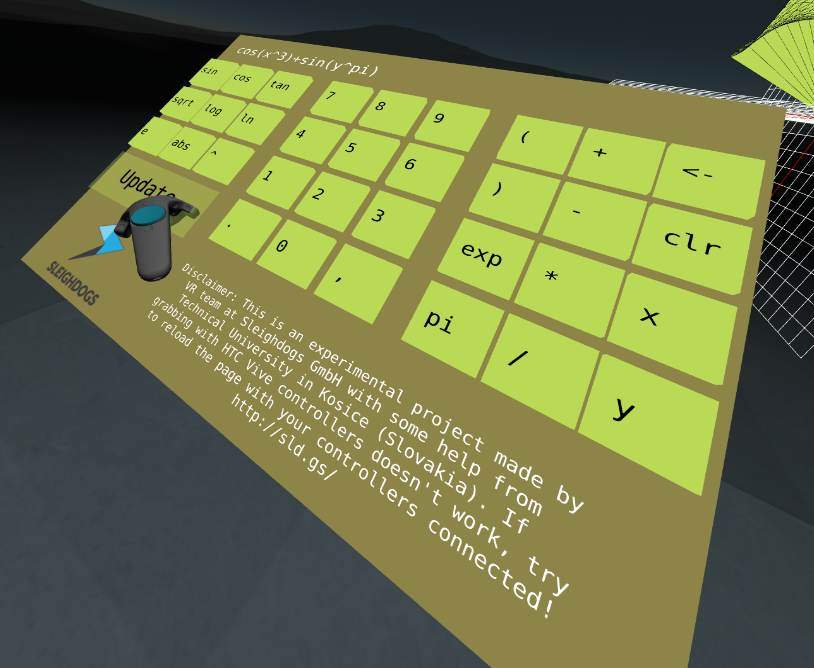
\includegraphics[width=0.7\textwidth]{calculator}
\caption{\textsl{Calculator} with multiple \textsl{CalcButton} components.}
\label{r:64}
\end{figure}

\subsection{ParametrizedFunction component}
First, the A-Frame API had to be extended with \texttt{parametricfunction} component:

\begin{lstlisting}[caption={Registering new A-Frame component \texttt{'parametricfunction'}.},captionpos=b]
AFRAME.registerComponent('parametricfunction', {
  schema: {/* ... */}, 
  init: function() {/* ... */},
  update: function() {/* ... */},
  remove: function() {/* ... */},
})
\end{lstlisting}

A-Frame components should have schema defined to ensure what data is passed into them. \texttt{parametricfunction}'s schema includes \texttt{equation}, \texttt{segments}, \texttt{xMin}, \texttt{xMax}, \texttt{yMin}, \texttt{yMax}, \texttt{zMin}, \texttt{zMax} and  \texttt{functionColor}, with their respective default values.

\begin{lstlisting}[caption={\texttt{parametricfunction} A-Frame component schema with default values.},captionpos=b]
schema: {
  equation: { type: 'string', default: '' },
  segments: { type: 'number', default: 20 },
  xMin: { type: 'number', default: -5 },
  xMax: { type: 'number', default: 5 },
  yMin: { type: 'number', default: -5 },
  yMax: { type: 'number', default: 5 },
  zMin: { type: 'number', default: -5 },
  zMax: { type: 'number', default: 5 },
  functionColor: { type: 'string', default: '#bada55' }
}
\end{lstlisting}

Main functions of \texttt{parametricfunction} A-Frame component are:
\begin{itemize}
\item{Parsing the equation passed into it with use of \texttt{Math.js} module and visualizing it in 3D environment, inside FunctionBox component that provides the grid.}
\item{Updating the 3D visualization after settings in \texttt{SettingsPanel} changes.}
\end{itemize}

\begin{lstlisting}[caption={Parsing of the equation.},captionpos=b]
var equation = 'f(x,y) = ' + this.data.equation;
var parser = math.parser();

try {
  parser.eval(equation);
} catch (error) {
  return;
}
\end{lstlisting}

To get the parsed value as a function, \texttt{parser.get('f')} method is called:

\begin{lstlisting}
const f1 = parser.get('f');
parser.clear();
\end{lstlisting}

The code of \texttt{parametricfunction} A-Frame component implementation is defined in \path{src/lib/components/parametricfunction.js}
    
\subsubsection{Action types}
ParametricFunction action types are defined in \path{src/actions/index.js} as string constants and exported individually to ensure they can be imported in other files and also tested.

\begin{lstlisting}[caption={\texttt{parametricFunction} action types.},captionpos=b]
export const PARAMETRIC_FUNCTION_SET_EQUATION = 'PARAMETRIC_FUNCTION_SET_EQUATION'
\end{lstlisting}

\subsubsection{Action creators}
ParametricFunction's action creators are pure functions that return payloads of information about type of \texttt{PARAMETRIC\char`_FUNCTION} action being dispatched and, if needed, also the data we want to send to Redux store. They are defined in \path{src/actions/index.js}

\begin{lstlisting}[caption={Action for setting the function for 3D visualization.},captionpos=b]
export const parametricFunctionSetEquation = (equation) => ({
  type: PARAMETRIC_FUNCTION_SET_EQUATION,
  equation,
})
\end{lstlisting}

\subsubsection{Initial state}
ParametricFunction component's initial state is defined inside the  \path{src/reducers/parametrizedFunction/index.js} file as a \texttt{initialState} object.

\begin{lstlisting}[caption={Initial state of a \textsl{calculator}.},captionpos=b]
const initialState = {
  equation: 'x^2 + y^2',
}
\end{lstlisting}

\subsubsection{Reducer function}
Reducer function for \texttt{ParametricFunction} component is defined in \path{src/reducers/parametricFunction/index.js}. From this file it's exported as a default function that takes state (with initialState as a default value) and action as its arguments and returns new state according to \texttt{PARAMETRIC\char`_FUNCTION} actions. Possible \texttt{ActionTypes} are conditionally checked with JavaScript's \texttt{switch} statement for a better code readability.

\begin{lstlisting}[caption={Update the \texttt{state.parametricFunction.equation} value.},captionpos=b]
export default (state = initialState, action) => {
  switch (action.type) {
    // ...
    case ActionTypes.PARAMETRIC_FUNCTION_SET_EQUATION:
      return { ...state, equation: action.equation }
   // ...
    default: return state
  }
}
\end{lstlisting}

\subsubsection{Higher-order component}
State and actions that ParametricFunction component needs to function properly are mapped to properties in ParametricFunction container - higher-order component. Code for ParametricFunction higher-order component creation is defined in \path{src/containers/ParametricFunction/index.js}.

\begin{lstlisting}[caption={Function to map \texttt{parametricFunction}  and \texttt{settings} state to component properties.},captionpos=b]
const mapStateToProps = (state) => ({
  equation: state.parametricFunction.equation,
  segments: state.settings.segments,
  xMin: state.settings.xMin,
  xMax: state.settings.xMax,
  yMin: state.settings.yMin,
  yMax: state.settings.yMax,
  zMin: state.settings.zMin,
  zMax: state.settings.zMax,
  functionColor: state.settings.functionColor,
})
\end{lstlisting}

\begin{lstlisting}[caption={Creation of \texttt{ParametricFunction} higher-order component.},captionpos=b]
import { connect } from 'react-redux'
import { ParametricFunction } from 'components'
// ...
export default connect(mapStateToProps)(ParametricFunction)
\end{lstlisting}

\subsubsection{Presentational component}
Presentational ParametricFunction component is implementing the \texttt{\justify parametricfunction} from A-Frame API we extended. Properties passed into the component as function attributes includes state and dispatchable action that was mapped in it's higher-order component. \texttt{ParametricFunction} code is defined in \path{src/components/ParametricFunction/index.js}.

\begin{lstlisting}[caption={Presentational \texttt{ParametricFunction} component code.},captionpos=b]
const ParametricFuntion = ({ equation, segments, xMin, xMax, yMin, yMax, zMin, zMax, functionColor }) => {
  return (
    <Entity
      id="function-mesh"
      parametricfunction={{
        equation,
        segments,
        xMin,
        xMax,
        yMin,
        yMax,
        zMin,
        zMax,
        functionColor,
      }}
      grid="size: 2; step: 20"
    />
  )
}
\end{lstlisting}

\subsection{FunctionBox component}
\subsubsection{Action types}
FunctionBox action types are defined in \path{src/actions/index.js} as string constants and exported individually to ensure they can be imported in other files and also tested.

\begin{lstlisting}[caption={\texttt{functionBox} action types.},captionpos=b]
export const FUNCTION_BOX_SET_POSITION = 'FUNCTION_BOX_SET_POSITION'
\end{lstlisting}

\subsubsection{Action creators}
FunctionBox's action creators are pure functions that return payloads of information about type of \texttt{FUNCTION\char`_BOX} action being dispatched and, if needed, also the data we want to send to Redux store. They are defined in \path{src/actions/index.js}

\begin{lstlisting}[caption={Action for setting function box position.},captionpos=b]
export const functionBoxSetPosition = (position) => ({
  type: FUNCTION_BOX_SET_POSITION,
  position,
})
\end{lstlisting}

\subsubsection{Initial state}
\texttt{FunctionBox} component's initial state is defined in \path{src/reducers/functionBox/index.js} as a \texttt{initialState} object.

\begin{lstlisting}[caption={Initial state of a \textsl{functionBox}.},captionpos=b]
const initialState = {
  position: { x: 0.65, y: 1.45, z: -1.03 },
}
\end{lstlisting}

\subsubsection{Reducer function}
Reducer function for \texttt{FunctionBox} component is defined in \path{src/reducers/functionBox/index.js}. From this file it's exported as a default function that takes state (with \texttt{initialState} as a default value) and \texttt{action} as its arguments and returns new state according to \texttt{FUNCTION\char`_BOX} actions. Possible \texttt{ActionTypes} are conditionally checked with JavaScript's \texttt{switch} statement for a better code readability.

\begin{lstlisting}[caption={Updating the   \texttt{state.functionBox.position} value.},captionpos=b]
export default (state = initialState, action) => {
  switch (action.type) {
    case ActionTypes.FUNCTION_BOX_SET_POSITION:
      return { ...state, position: action.position }
    default: return state
  }
}
\end{lstlisting}

\subsubsection{Higher-order component}
State and actions that \texttt{FunctionBox} component needs to function properly are mapped to properties in Calculator container -  higher-order component. Code for FunctionBox higher-order component creation is defined in \path{src/containers/FunctionBox/index.js}.

\begin{lstlisting}[caption={Function to map \texttt{functionBox} state to component properties.},captionpos=b]
const mapStateToProps = (state) => ({
  position: state.functionBox.position,
})
\end{lstlisting}

\begin{lstlisting}[caption={Creation of \texttt{FunctionBox} higher-order component.},captionpos=b]
import { connect } from 'react-redux'
import { FunctionBox } from 'components'
// ...
export default connect(mapStateToProps, null)(FunctionBox)
\end{lstlisting}

\subsubsection{Presentational component}
Presentational FunctionBox component is implementing the \texttt{geometry} and \texttt{material} from A-Frame API. It's shape is determined by \texttt{geometry.primitive} which is set to \texttt{'box'} with width of \texttt{4} meters, height of \texttt{4} meters and depth of \texttt{4} meters. By default it's scaled down by 80\%, but since this component is interactive, it can be stretched with hand controller interactions. It can also be moved around the 3D environment. \texttt{Position} property is passed into the component from higher-order component. \texttt{FunctionBox} code is defined in \path{src/components/FunctionBox/index.js}.

\begin{lstlisting}[caption={Presentational \textsl{FunctionBox} component code.},captionpos=b]
const FunctionBox = ({ position, ...props }) => (
  <Entity
    id="function-box"
    className="interactive"
    geometry="primitive: box; width: 4; height: 4; depth: 4;"
    material="transparent: true; opacity: 0; shader: standard"
    scale="0.2 0.2 0.2"
    position={position}
    grabbable
    stretchable
    dynamic-body
    stop-flying
  >
    { props.children }
  </Entity>
)  
\end{lstlisting}

\subsection{SettingsPanel component}
First, the A-Frame API has to be extended with \texttt{datgui} component. Inside its \texttt{init} method, the \texttt{dat.guiVR} instance is created and injected into the component element property:

\begin{lstlisting}
const gui = dat.GUIVR.create( this.data.name );
this.el.setObject3D('gui', gui );
this.el.gui = gui;
\end{lstlisting}

To allow VR hand controllers interactions, \texttt{bindInput} method is used for creation of event listeners for \texttt{triggerdown}, \texttt{triggerup}, \texttt{gripdown} and \texttt{gripup} events:

\begin{lstlisting}
function bindInput(el, input) {
  el.addEventListener('triggerdown', function() {
    input.pressed(true);
  });
  el.addEventListener('triggerup', function() {
    input.pressed(false);
  });
  el.addEventListener('gripdown', function() {
    input.gripped(true);
  });
  el.addEventListener('gripup', function() {
    input.gripped(false);
  });
}
\end{lstlisting}

\subsubsection{Action types}
SettingsPanel action types are defined in \path{src/actions/index.js} as string constants and exported individually to ensure they can be imported in other files and also tested.

\begin{lstlisting}[caption={\texttt{settings} action types.},captionpos=b]
export const SETTINGS_SET_X_MIN = 'SETTINGS_SET_X_MIN'
export const SETTINGS_SET_Y_MIN = 'SETTINGS_SET_Y_MIN'
export const SETTINGS_SET_Z_MIN = 'SETTINGS_SET_Z_MIN'
export const SETTINGS_SET_X_MAX = 'SETTINGS_SET_X_MAX'
export const SETTINGS_SET_Y_MAX = 'SETTINGS_SET_Y_MAX'
export const SETTINGS_SET_Z_MAX = 'SETTINGS_SET_Z_MAX'
export const SETTINGS_SET_SEGMENTS = 'SETTINGS_SET_SEGMENTS'
export const SETTINGS_SET_FUNCTION_COLOR = 'SETTINGS_SET_FUNCTION_COLOR'
\end{lstlisting}

\subsubsection{Action creators}
SettingsPanel's action creators are pure functions that return payloads of information about type of \texttt{SETTINGS} action being dispatched and, if needed, also the data we want to send to Redux store. They are defined in \path{src/actions/index.js}

\begin{lstlisting}[caption={Action for setting fnction segments.},captionpos=b]
export const settingsSetSegments = (segments) => ({
  type: SETTINGS_SET_SEGMENTS,
  segments,
})
\end{lstlisting}

\subsubsection{Initial state}
SettingsPanel component's initial state is defined in \path{src/reducers/settings/index.js} as a \texttt{initialState} object.

\begin{lstlisting}[caption={Initial state of a \textsl{calculator}.},captionpos=b]
const initialState = {
  xMin: -1,
  yMin: -1,
  zMin: -4,
  xMax: 1,
  yMax: 1,
  zMax: 4,
  segments: 30,
  functionColor: '#bada55',
}
\end{lstlisting}

\subsubsection{Reducer function}
Reducer function for \texttt{SettingsPanel} component is defined in \path{src/reducers/settings/index.js}. From this file it's exported as a default function that takes state (with initialState as a default value) and action as its arguments and returns new state according to \texttt{SETTINGS} actions. Possible \texttt{ActionTypes} are conditionally checked with JavaScript's \texttt{switch} statement for a better code readability.

\begin{lstlisting}[caption={Update of \texttt{state.settings.segments} value.},captionpos=b]
export default (state = initialState, action) => {
  switch (action.type) {
    // ...
    case ActionTypes.SETTINGS_SET_SEGMENTS:
      return { ...state, segments: action.segments }
   // ...
    default: return state
  }
}
\end{lstlisting}

\subsubsection{Higher-order component}
State and actions that SettingsPanel component needs to function properly are mapped to properties in SettingsPanel container - higher-order component. Code for SettingsPanel higher-order component creation is defined in \path{src/containers/SettingsPanel/index.js}.

\begin{lstlisting}[caption={Function to map dispatchable \texttt{settings} action creators to component properties.},captionpos=b]
const mapDispatchToProps = (dispatch) => {
  return {
    setXMin: (xMin) => dispatch(settingsSetXMin(xMin)),
    setYMin: (yMin) => dispatch(settingsSetYMin(yMin)),
    setZMin: (zMin) => dispatch(settingsSetZMin(zMin)),
    setXMax: (xMax) => dispatch(settingsSetXMax(xMax)),
    setYMax: (yMax) => dispatch(settingsSetYMax(yMax)),
    setZMax: (zMax) => dispatch(settingsSetZMax(zMax)),
    setSegments: (segments) => dispatch(settingsSetSegments(segments)),
    setFunctionColor: (color) => dispatch(settingsSetFunctionColor(color)),
  }
}
\end{lstlisting}

\begin{lstlisting}[caption={Creation of \texttt{SettingsPanel} higher-order component.},captionpos=b]
import { connect } from 'react-redux'
import { SettingsPanel } from 'components'
// ...
export default connect(null, mapDispatchToProps)(SettingsPanel)
\end{lstlisting}

\subsubsection{Presentational component}
Presentational SettingsPanel component is implementing the \texttt{datgui} from A-Frame API that we extended. Individual settings are handled by \texttt{SettingsController} component, which triggers the action when user changes the value by pointing to the settings with VR hand controller and pressing the trigger button. \texttt{SettingsPanel} code is defined in \path{src/components/SettingsPanel/index.js}.

\begin{lstlisting}[caption={Presentational \textsl{Calculator} component code.},captionpos=b]
const SettingsPanel = ({
  name,
  controllerLeft,
  controllerRight,
  setSegments,
  ...props
}) => {
  return (
    <Entity datgui={{ name, controllerLeft, controllerRight }} {...props}>
      <SettingsController type="slider" name="segments" step={1} min={1} max={50} initialState={30} actionToTrigger={setSegments} />
      { /* ...other settings... */ }
    </Entity>
  )
} 
\end{lstlisting}

\begin{figure}[ht!]
\centering
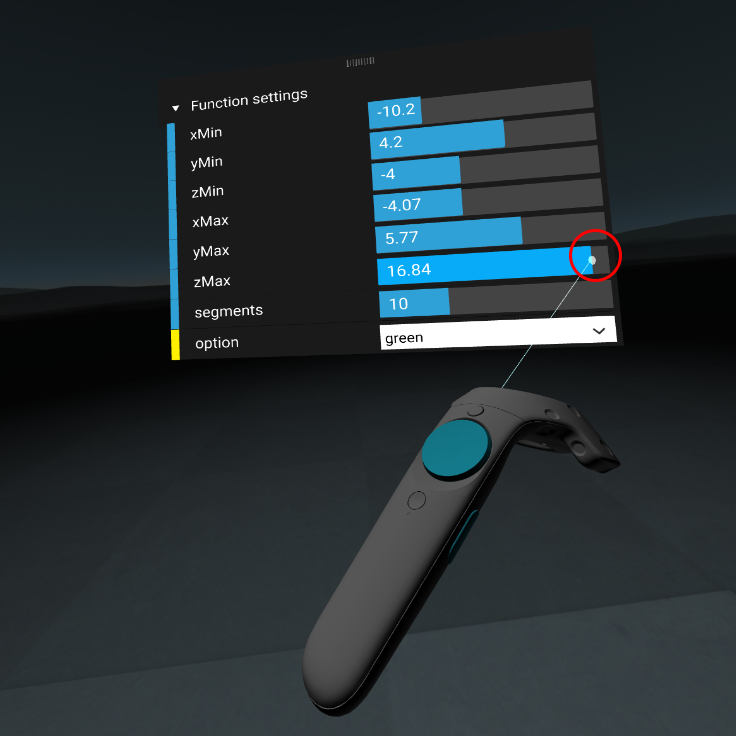
\includegraphics[width=0.8\textwidth]{function_settings}
\caption{\texttt{SettingsPanel} component}
\label{r:65}
\end{figure}

\newpage
\subsection{Hand controller components}
VR hand controllers implement the \texttt{super-hands} A-Frame API that was extended by importing the \texttt{aframe-super-hands-component} in MathworldVR's \texttt{VRScene} component. \texttt{super-hands} A-Frame component adds natural, intuitive hand controller interactions, interprets input from tracked controllers and collision detection into interaction gestures and communicates those gestures to target entities for them to respond.

The currently implemented gestures are:
\begin{itemize}
\item{Hover - Holding a controller in the collision space of an entity.}
\item{Grab - Pressing a button while hovering an entity, potentially also moving it.}
\item{Stretch - Grabbing an entity with two hands and resizing.}
\item{Drag-drop - Dragging an entity onto another entity.}
\end{itemize}

\texttt{super-hand} includes components for typical reactions to the implemented gestures: \texttt{hoverable}, \texttt{grabbable}, \texttt{stretchable}, and \texttt{drag-droppable}. Code for hand controllers implementation used in MathworldVR is defined in \path{src/components/LeftController/index.js} and \path{src/components/LeftController/index.js} respectively.

\begin{figure}[ht!]
\centering
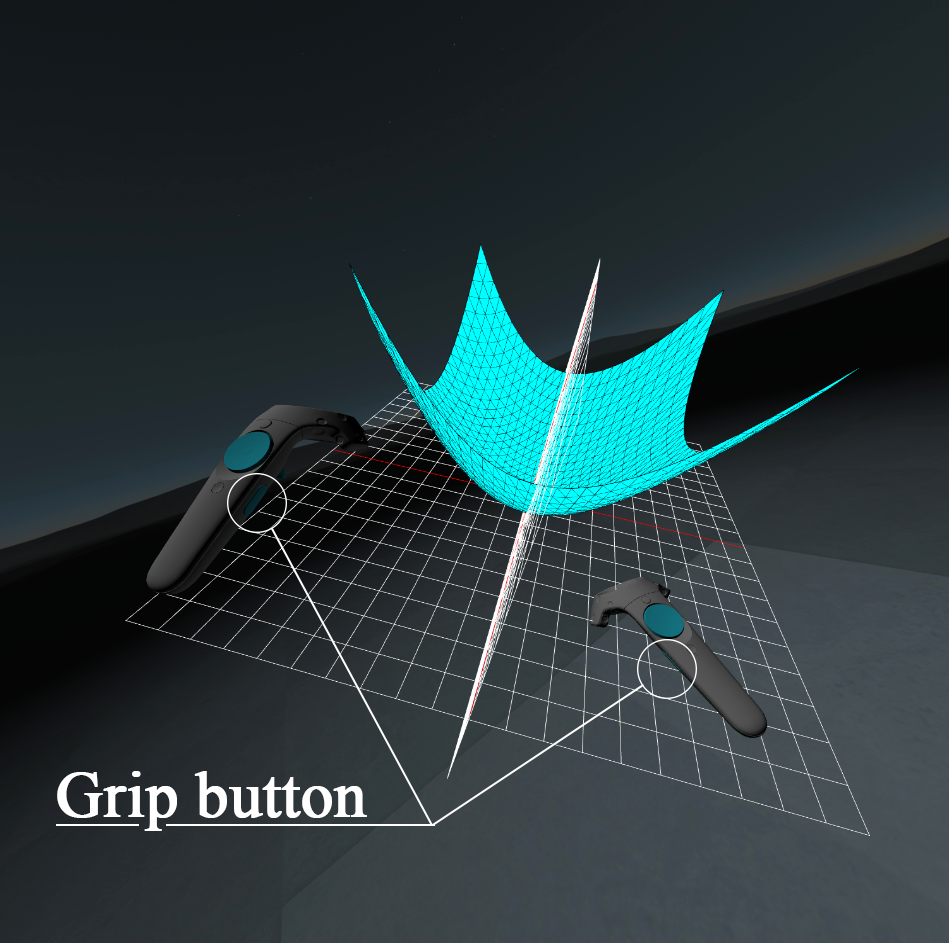
\includegraphics[width=0.7\textwidth]{grab}
\caption{Grabbing functionality}
\label{r:5}
\end{figure}

\begin{figure}[ht!]
\centering
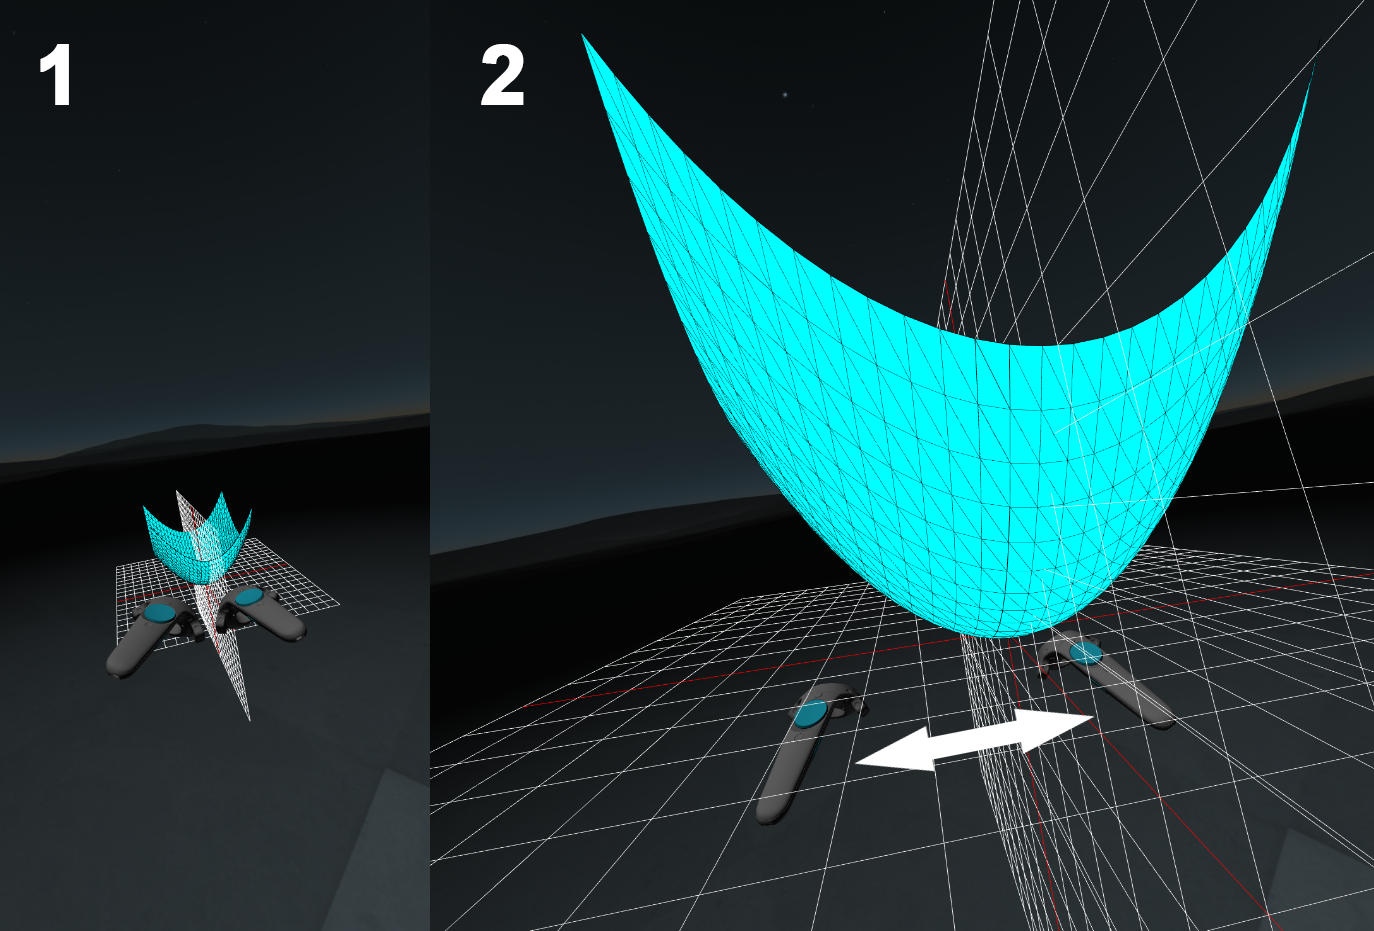
\includegraphics[width=0.7\textwidth]{scaling}
\caption{Scaling functionality}
\label{r:6}
\end{figure}

\newpage
\subsection{AttentionBox component}
\texttt{AttentionBox} component is used for displaying semi-transparent rectangle with MathworldVR project information in the middle of the browser screen. \texttt{AttentionBox} component is defined in \path{src/components/AttentionBox/index.js}.

\subsection{Adding components into A-Frame scene}
To add MathworldVR components into the 3D environment, they need to be included as a children components of \texttt{VRScene} component:

\begin{lstlisting}
<VRScene>
  <AttentionBox />
  <LeftController />
  <RightController />

  <FunctionBox>
    <ParametricFunction />
  </FunctionBox>

  <Calculator />

  <SettingsPanel
    name="Function settings"
    position={{ x: -0.37, y: 1.93, z: -0.34 }}
    rotation={{ x: 10, y: 30, z: 0 }}
    scale={{ x: 0.5, y: 0.5, z: 0.5 }}
  />

  <Sky />
  <Lights />
  <Plane />
</VRScene>
\end{lstlisting}

\subsection{Building and deploying the application to web hosting}
Application's JavaScript code is bundled together by using NPM script \texttt{npm run build}, which produces production-ready bundle. Build script triggers pre-build task, which gets executed before the build and consists of  \texttt{npm run build:clean} (for removing all files from \texttt{/build} folder) and \texttt{npm run build:copy} (for copying static files like \texttt{index.html}, assets, images, CSS stylesheets into cleaned \texttt{/build} folder) scripts, called synchronously.

To deploy the application, \texttt{/build} folder contents are copied to the server, hosted on \url{https://www.fortrabbit.com/}. Hosting is sponsored by \textsl{Sleighdogs, GmbH} company, which author is working for during writing of this thesis. Server us hosted under \url{http://vr.sld.gs/mathworldvr/} domain.

\newpage

\begin{figure}[ht!]
\centering
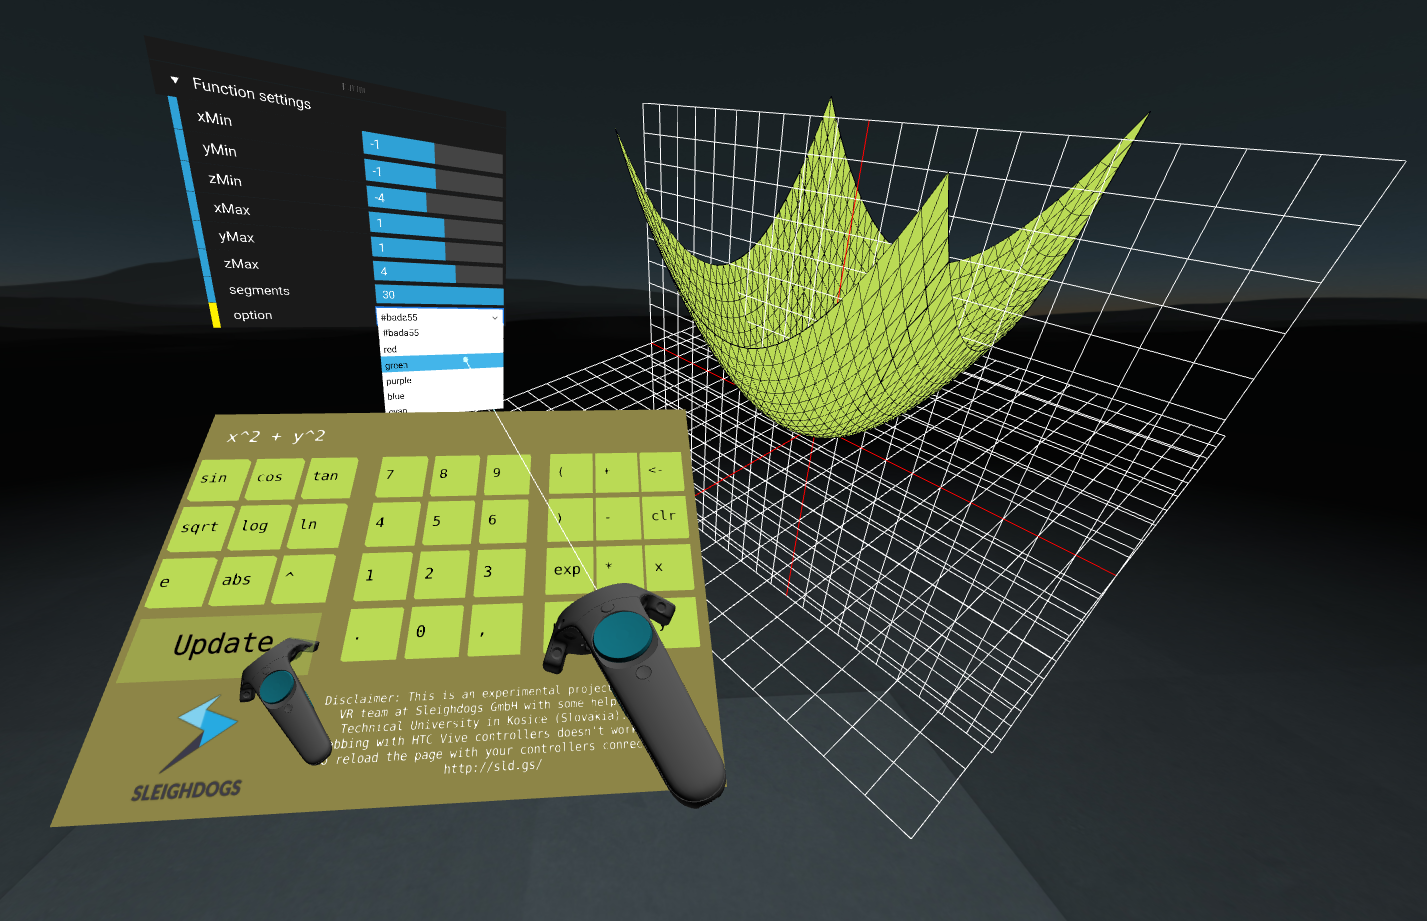
\includegraphics[width=1\textwidth]{main}
\caption{Finalized MathworldVR application, deployed on live server.}
\label{r:69}
\end{figure}

